\section{Exploratory Data Analysis (EDA)}
The original dataset comprises data from 390 subjects. However, some of them have missing values in some variables. Since the proposed Bayesian model requires complete cases for all predictors, a data cleaning process was performed by removing observations with incomplete entries. As a result, the effective sample size used for this analysis consists of 367 subjects (approximately 94\% of the original sample). The response variable is GHB, and the potential predictors include Stabilized Glucose (SGLU) among others. All statistical analyses and visualisations were conducted using R programming language \cite{rstat}.

\begin{figure}[h!]
	\centering
	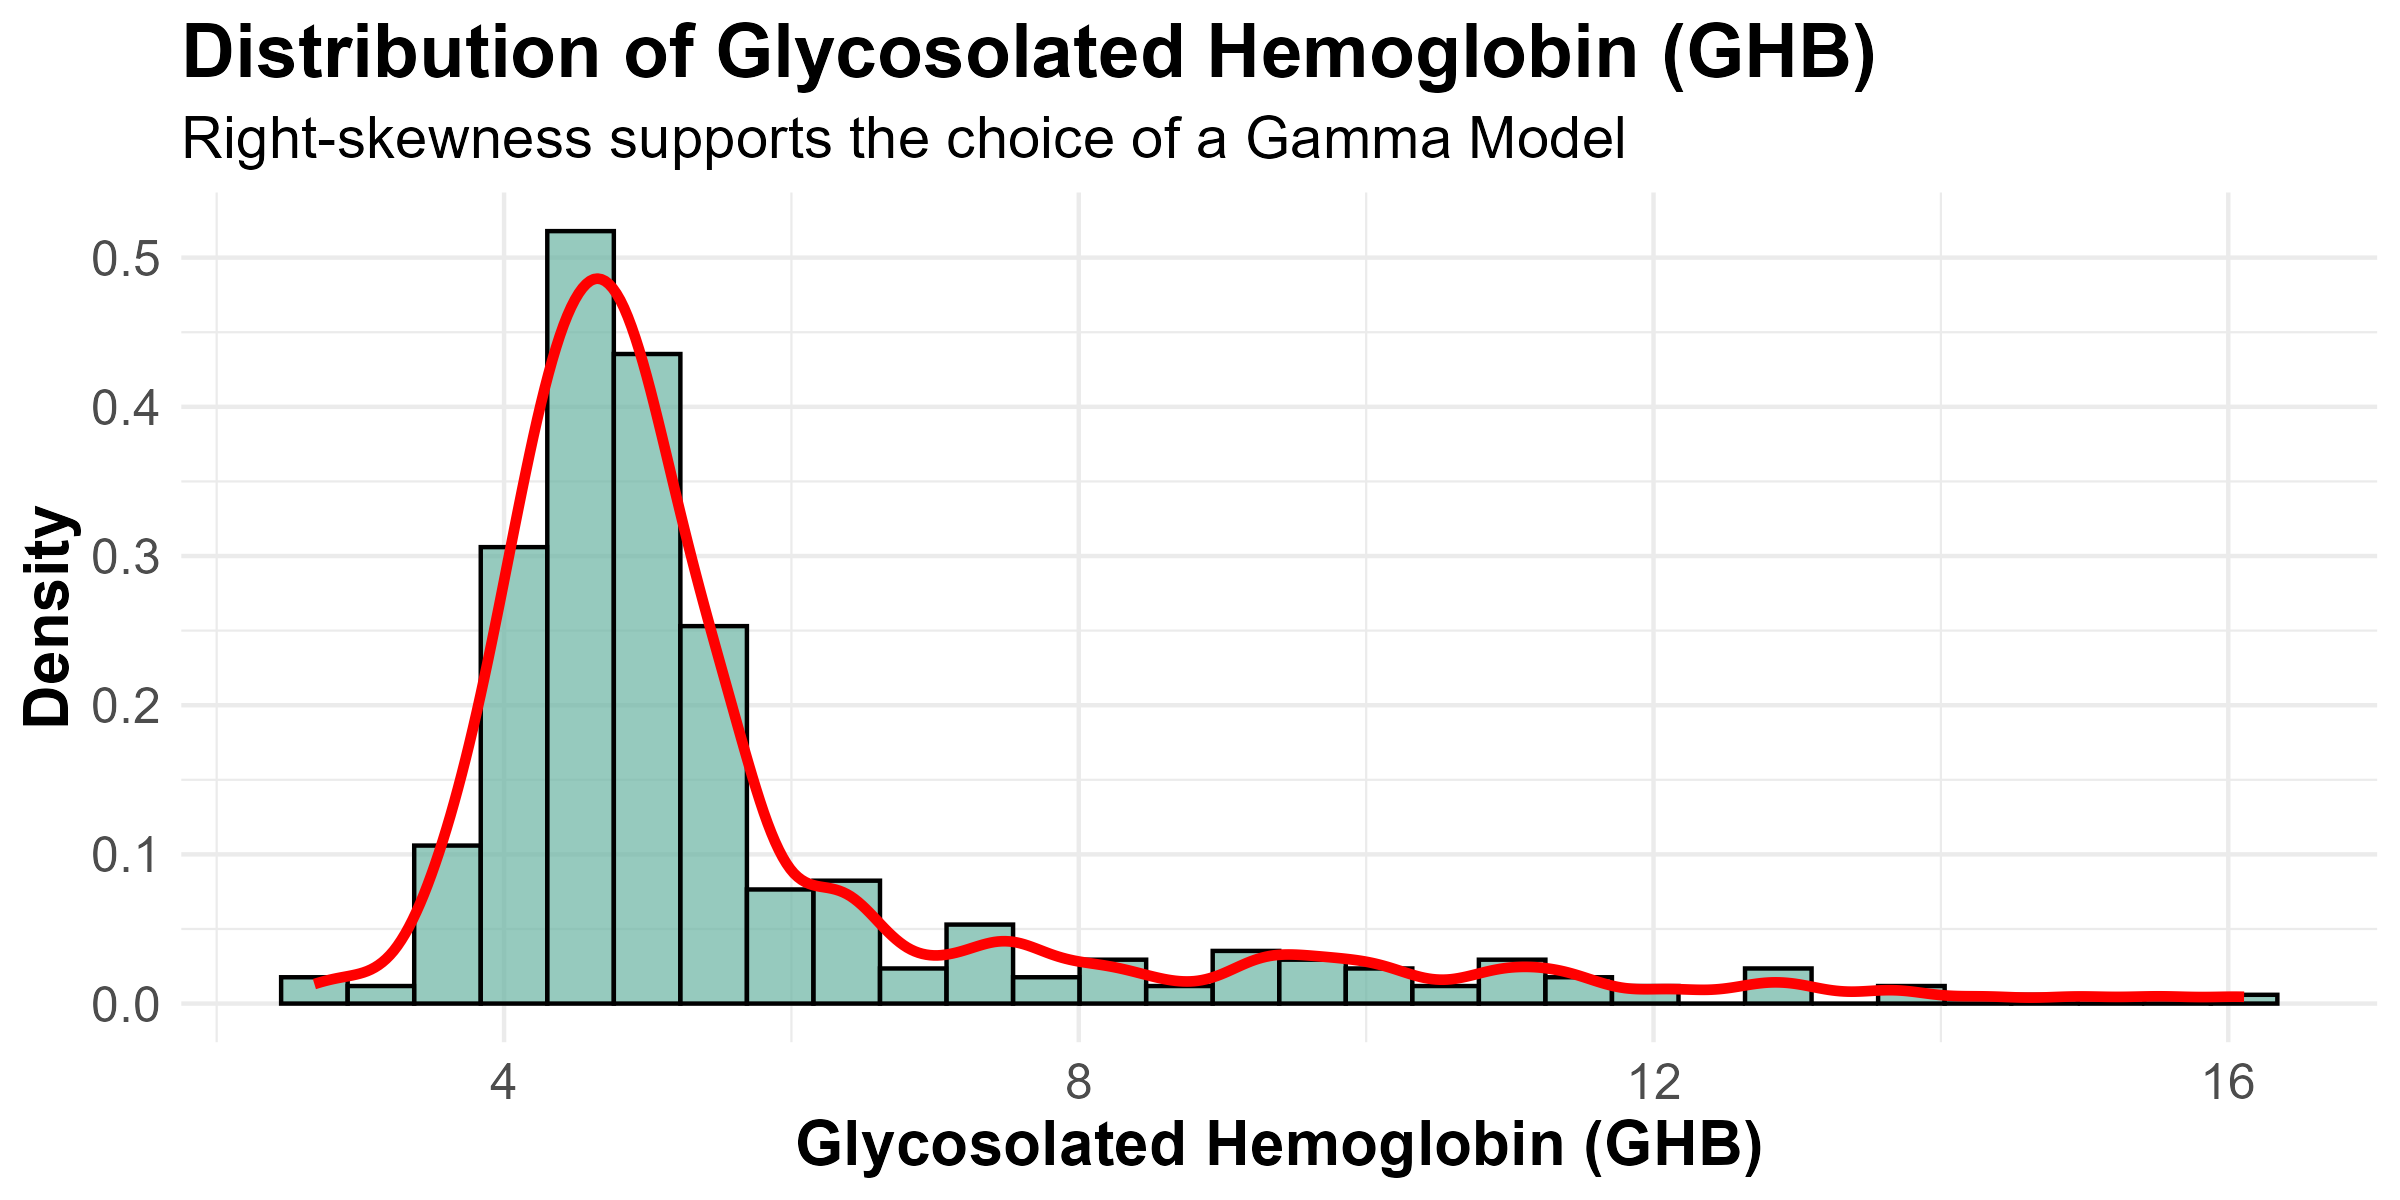
\includegraphics[width=0.63\linewidth]{Figures/histogram_ghb}
	\caption{Histogram and density estimate of GHB levels.}
	\label{fig:histogramghb}
\end{figure}
As observed in Figure (\ref{fig:histogramghb}), the distribution of GHB is asymmetric with a long right tail (positive skewness), with only positive values. This observation confirms that a Normal distribution would be a poor fit for the data and supports the choice of a Gamma distribution, which is ideal for modeling continuous, positive, and skewed data \cite{silva2023notes}.
\begin{figure}[h!]
	\centering
	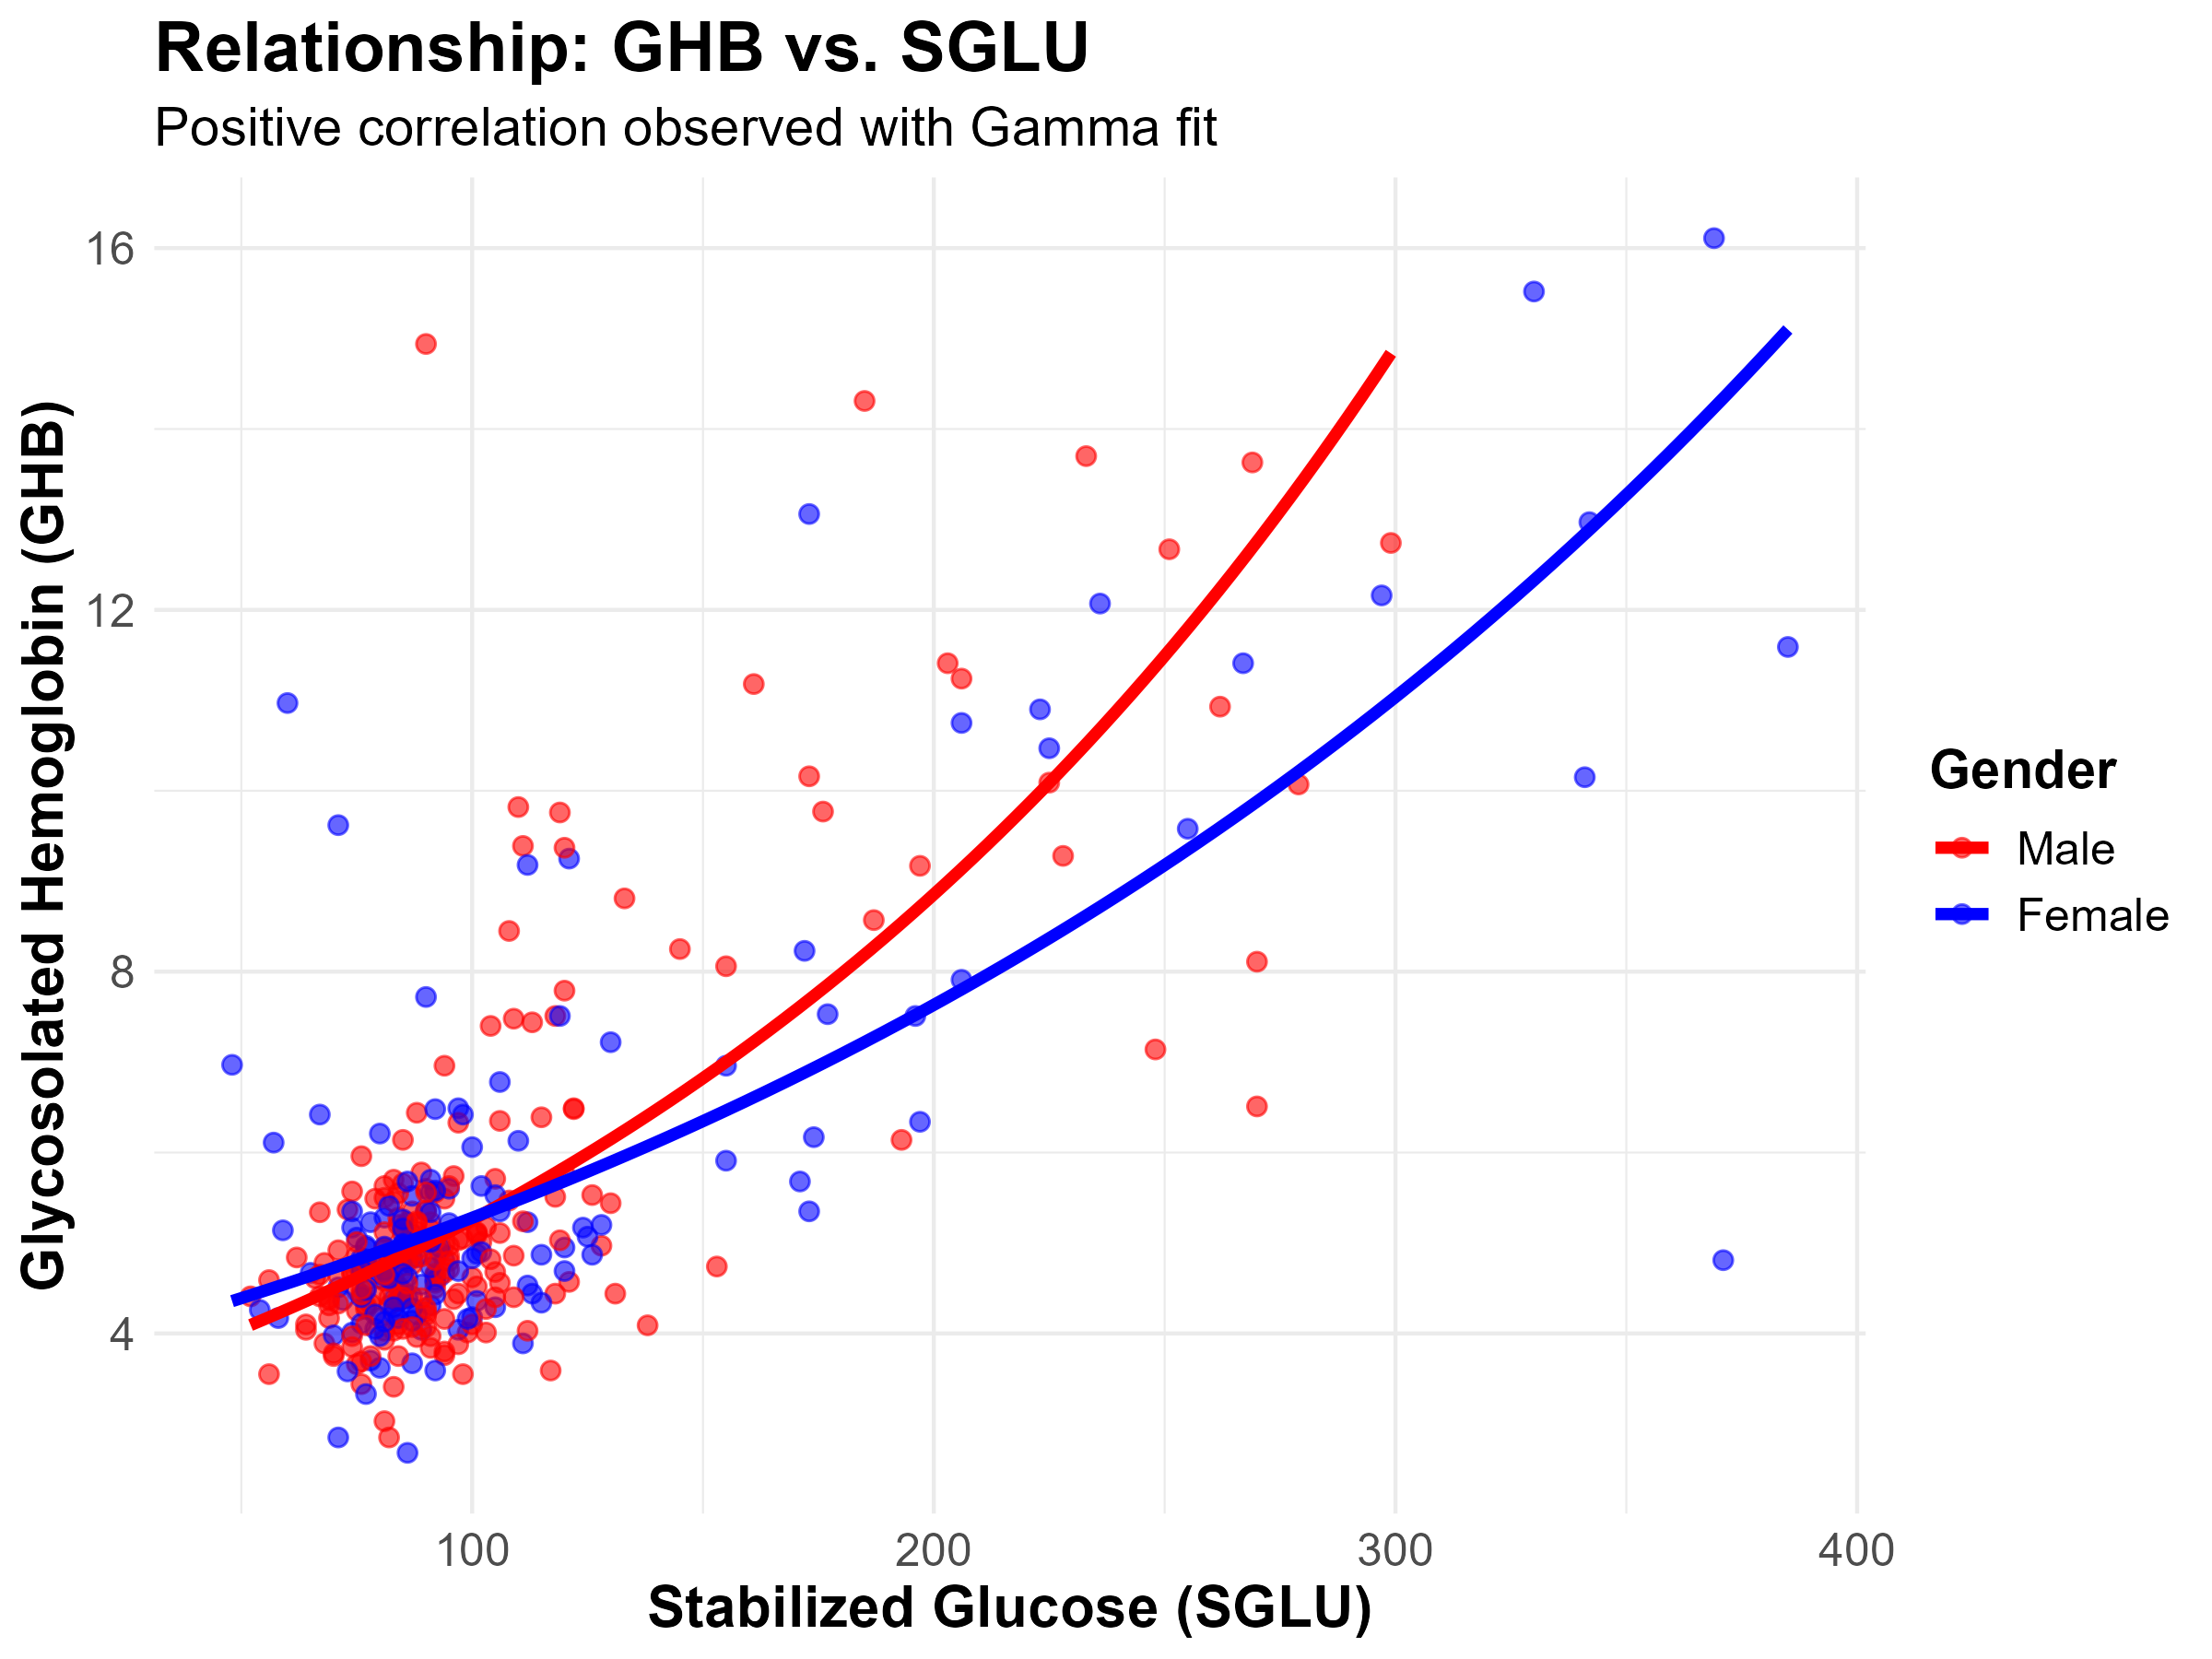
\includegraphics[width=0.54\linewidth]{Figures/scatterplot_glucose}
	\caption{Scatter plot of GHB against SGLU, stratified by gender.}
	\label{fig:scatterplotglucose}
\end{figure}

Figure (\ref{fig:scatterplotglucose}) illustrates the relationship between GHB and SGLU. There is a visible positive trend: as glucose levels increase, GHB levels also tend to rise. This suggests that SGLU will likely be a significant predictor in our regression model. No obvious clustering was found regarding the Location variable (Buckingham vs. Louisa), suggesting geographic factors might not be significant. Although the plot distinguishes between male and female subjects, the fitted regression curves for both groups appear to follow a very similar trajectory/slope. 

\begin{figure}[h!]
	\centering
	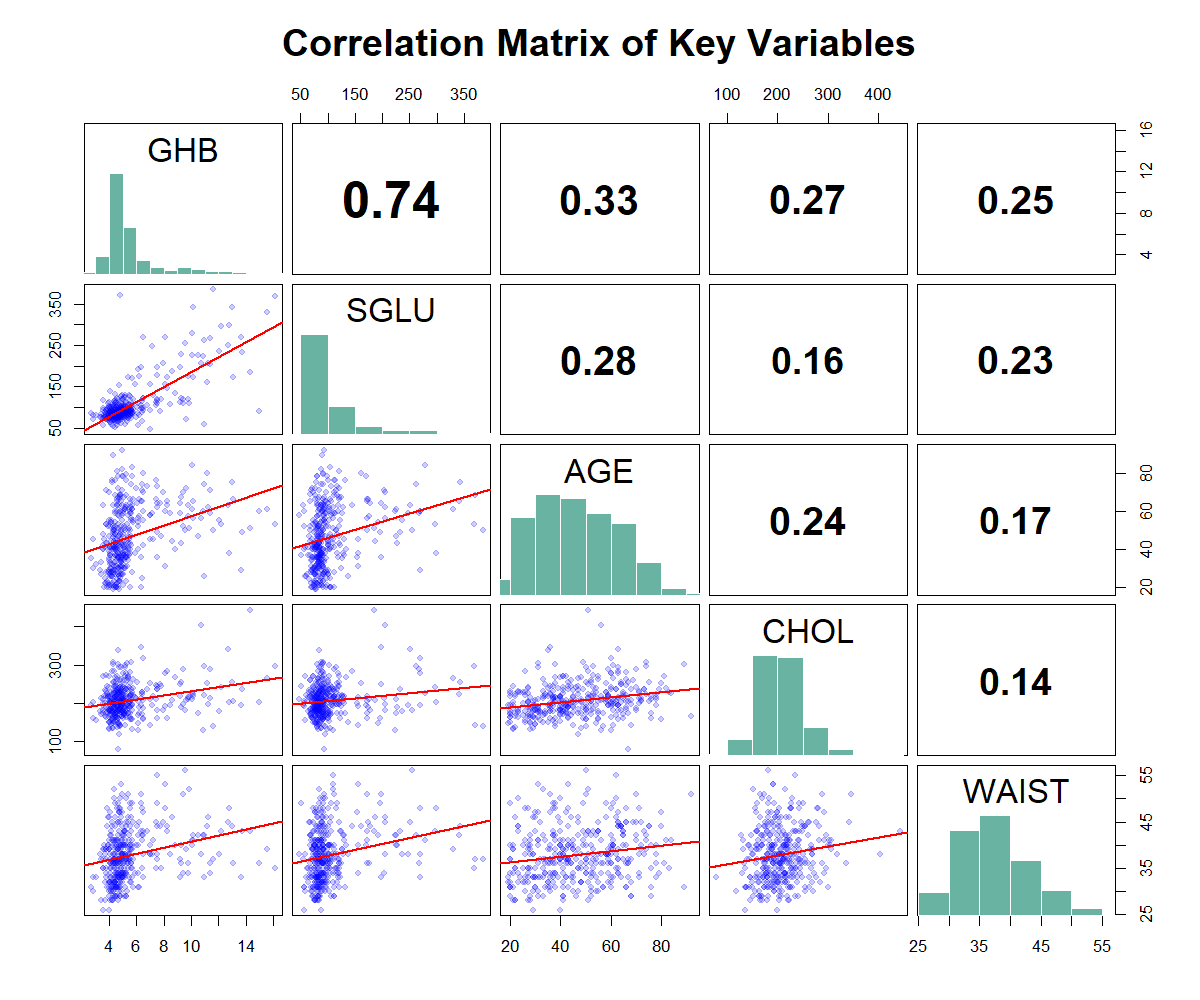
\includegraphics[width=0.65\linewidth]{Figures/correlation_matrix_final_large}
	\caption{Matrix of pairwise scatter plots, histograms, and Pearson correlation coefficients for the response variable (GHB) and key predictors.}
	\label{fig:correlationmatrixfinallarge}
\end{figure}

To investigate multicollinearity and secondary predictors, a Pearson correlation matrix was generated (Figure (\ref{fig:correlationmatrixfinallarge})). To avoid ambiguity with the Gamma shape parameter ($r$), we denote the sample correlation coefficient as $c$. Based on the multivariate analysis, a selection criterion was established to retain predictors showing a correlation of at least 0.20 ($c \ge 0.20$) with the response variable. Applying this threshold, the following variables were selected for the Bayesian regression model: SGLU, Age, Cholesterol, Waist Circumference and Systolic Blood Pressure (SBP) (the full correlation matrix (Appendix (\ref{app:apexA})) confirms that SBP also meets the inclusion threshold). This data-driven selection ensures that the model focuses on factors with meaningful associations with GHB.

\begin{figure}[h!]
	\centering
	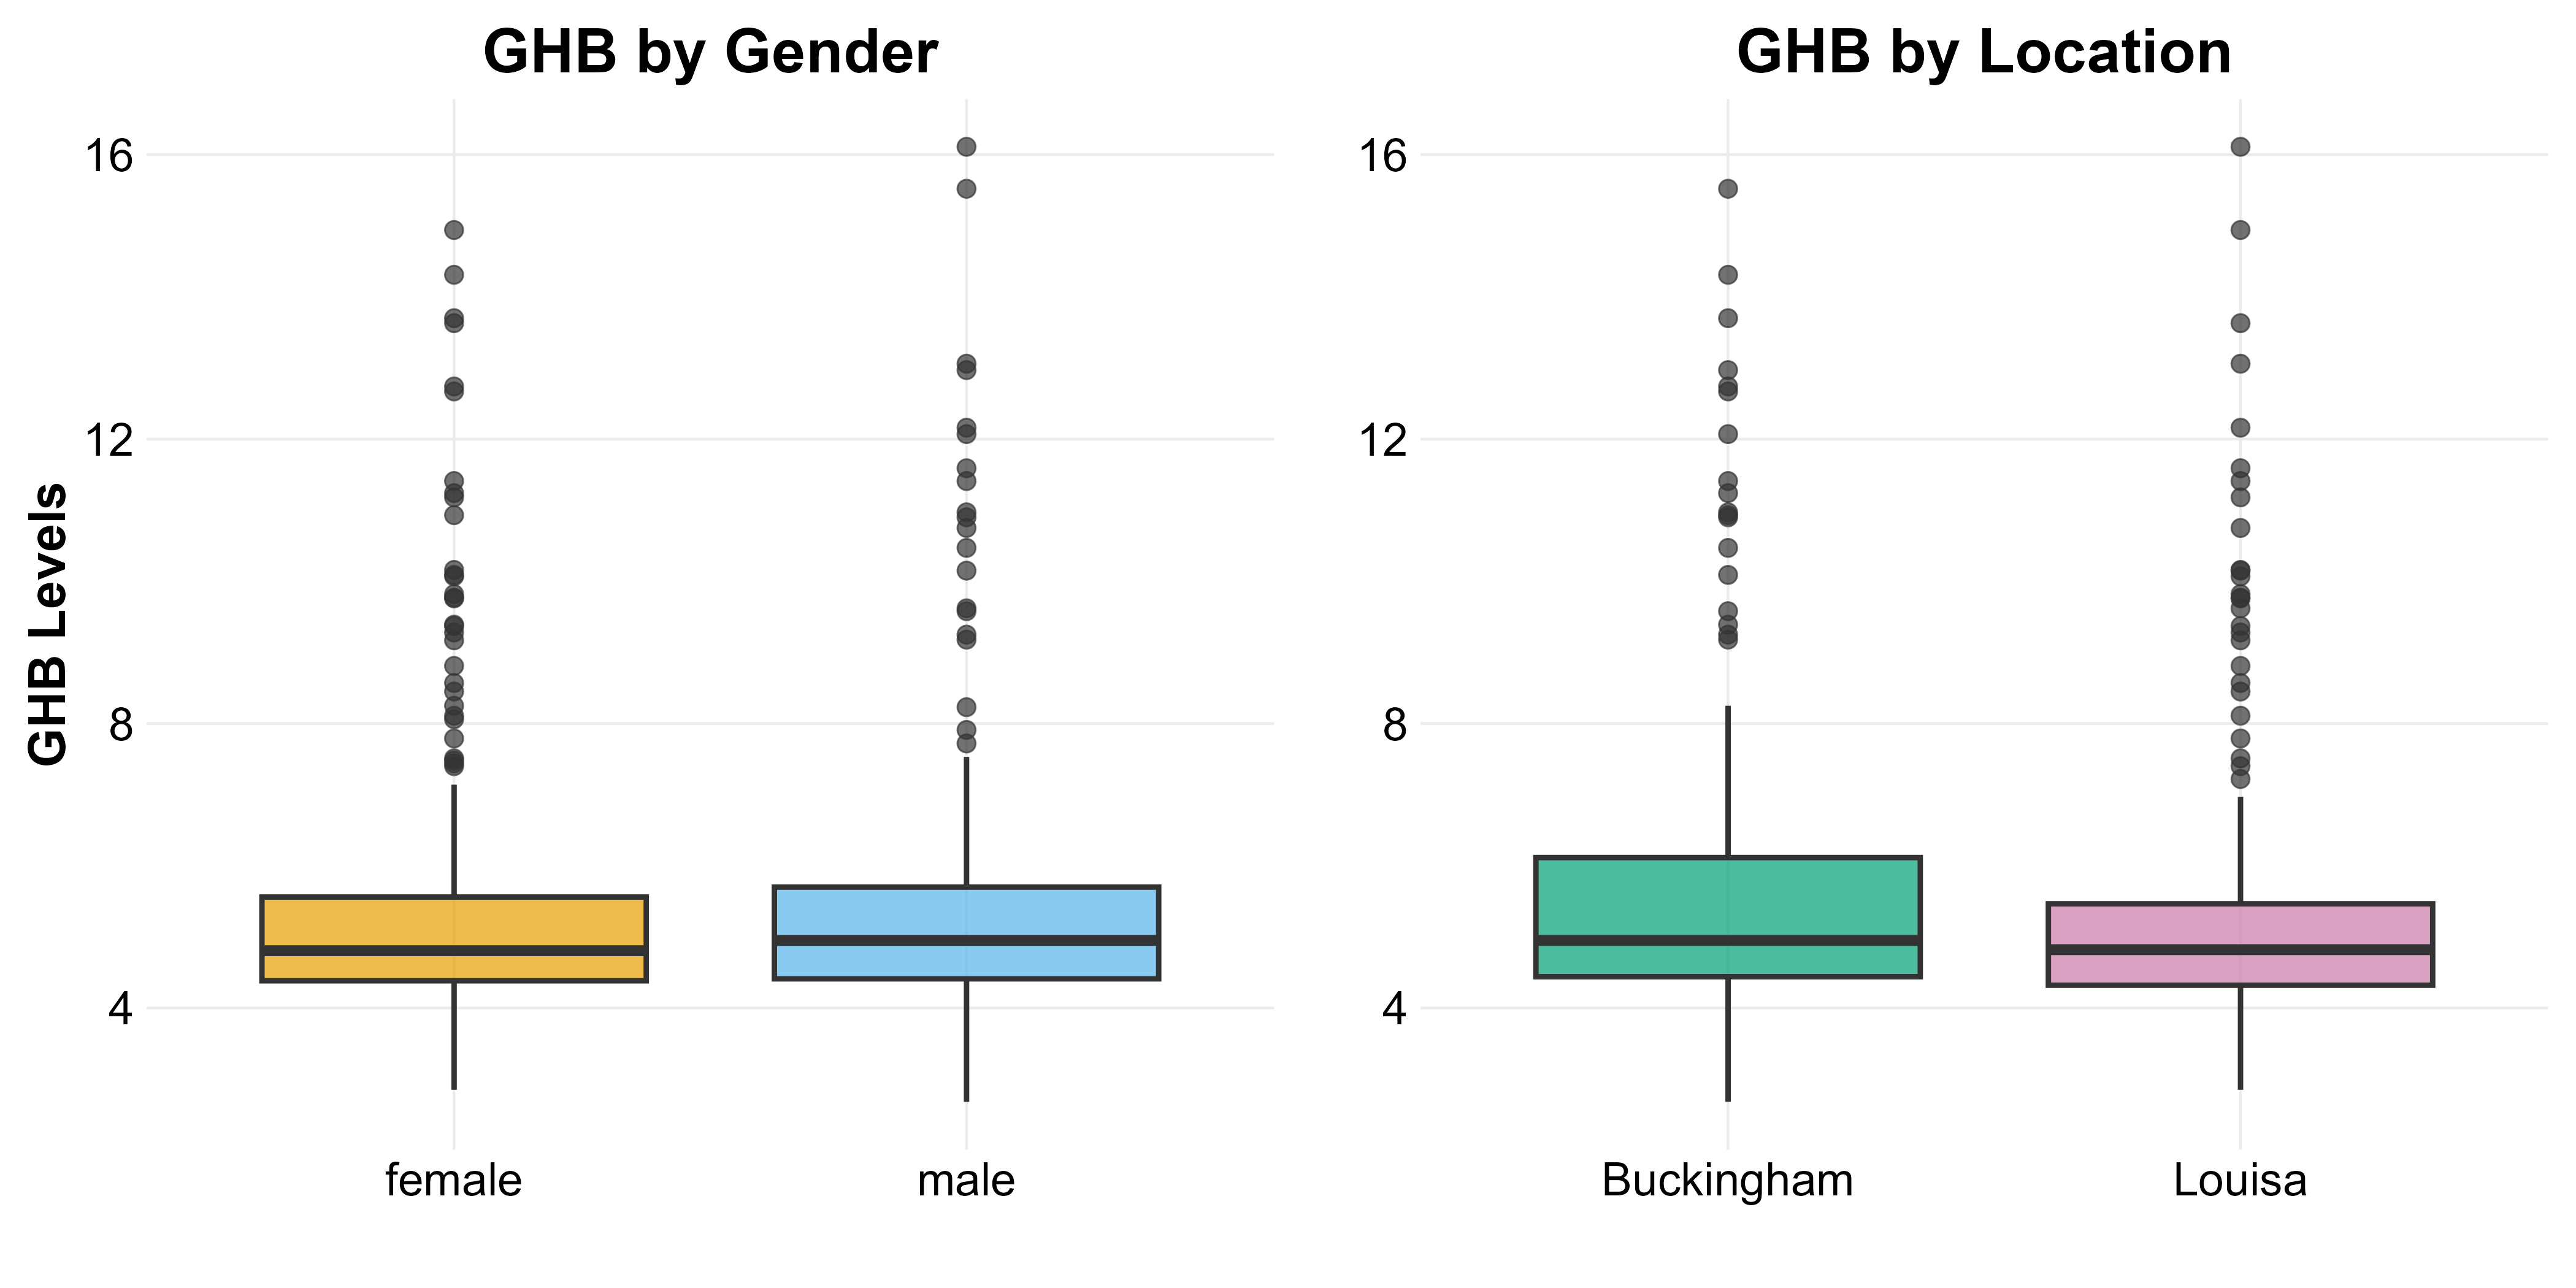
\includegraphics[width=0.7\linewidth]{Figures/boxplots_categorical}
	\caption{Boxplots of GHB levels stratified by demographic factors: Gender (left) and Location (right).}
	\label{fig:boxplotscategorical}
\end{figure}
To assess the potential impact of demographic factors, we analyzed the distribution of GHB across Gender and Location using boxplots (Figure (\ref{fig:boxplotscategorical})). The median GHB levels are very similar for females and males. The interquartile ranges also show significant overlap, suggesting that gender is not a strong differentiator. Similarly, the distribution of GHB levels appears consistent between subjects from Buckingham and Louisa. Both plots reveal the presence of high-value outliers, indicating subjects with severe diabetic conditions across all demographic groups. Neither gender nor location are primary driver of GHB levels.





